
\documentclass[letterpaper,11pt]{article}

% Choose bibliography style for formatting list of publications
\usepackage[style=ieee,url=false,doi=false,maxbibnames=99,sorting=ydnt,dashed=false]{biblatex}
\bibliography{papers}

% Choose theme, e.g. black, RedViolet, ForestGreen, MidnightBlue
\def\theme{black}

% More predefined colors can be found in 
% https://en.wikibooks.org/wiki/LaTeX/Colors
% Example photograph taken from Wikimedia Commons
% https://commons.wikimedia.org/wiki/File:Kiara_Krit_passport.jpg

\usepackage{simplecv}
\usepackage{import}
\usepackage{pdfpages}

\boldname{Huang}{Yingsheng}{Y.}

\begin{document}

% Heading
\headinginline{Yingsheng Huang}{
    Email: \email{huangys@ihep.ac.cn} \\
    INSPIRE ID: {\href{https://inspirehep.net/authors/1716525}{Ying.Sheng.Huang.1}} \\ 
    ORCID: {\href{https://orcid.org/0000-0002-9394-0688}{0000-0002-9394-0688}}\\
    % LinkedIn: \linkedin{name-surname} \\
    % GitHub: \github{example}
    Phone: +86 156 1156 3739
}

% \headingphoto{Name Surname}{
% %     Website: \website{example.com} \\ 
%     Email: \email{huangys@ihep.ac.cn} \\
% %     LinkedIn: \linkedin{name-surname} \\
% %     GitHub: \github{example}
% }{photo.jpg}

% Page One
\import{sections/}{education.tex}
% \import{sections/}{experience.tex}
\import{sections/}{statement.tex}

% \pagebreak

\import{sections/}{publications.tex}
% \pagebreak
\import{sections/}{talks.tex}

\import{sections/}{references.tex}

\pagebreak

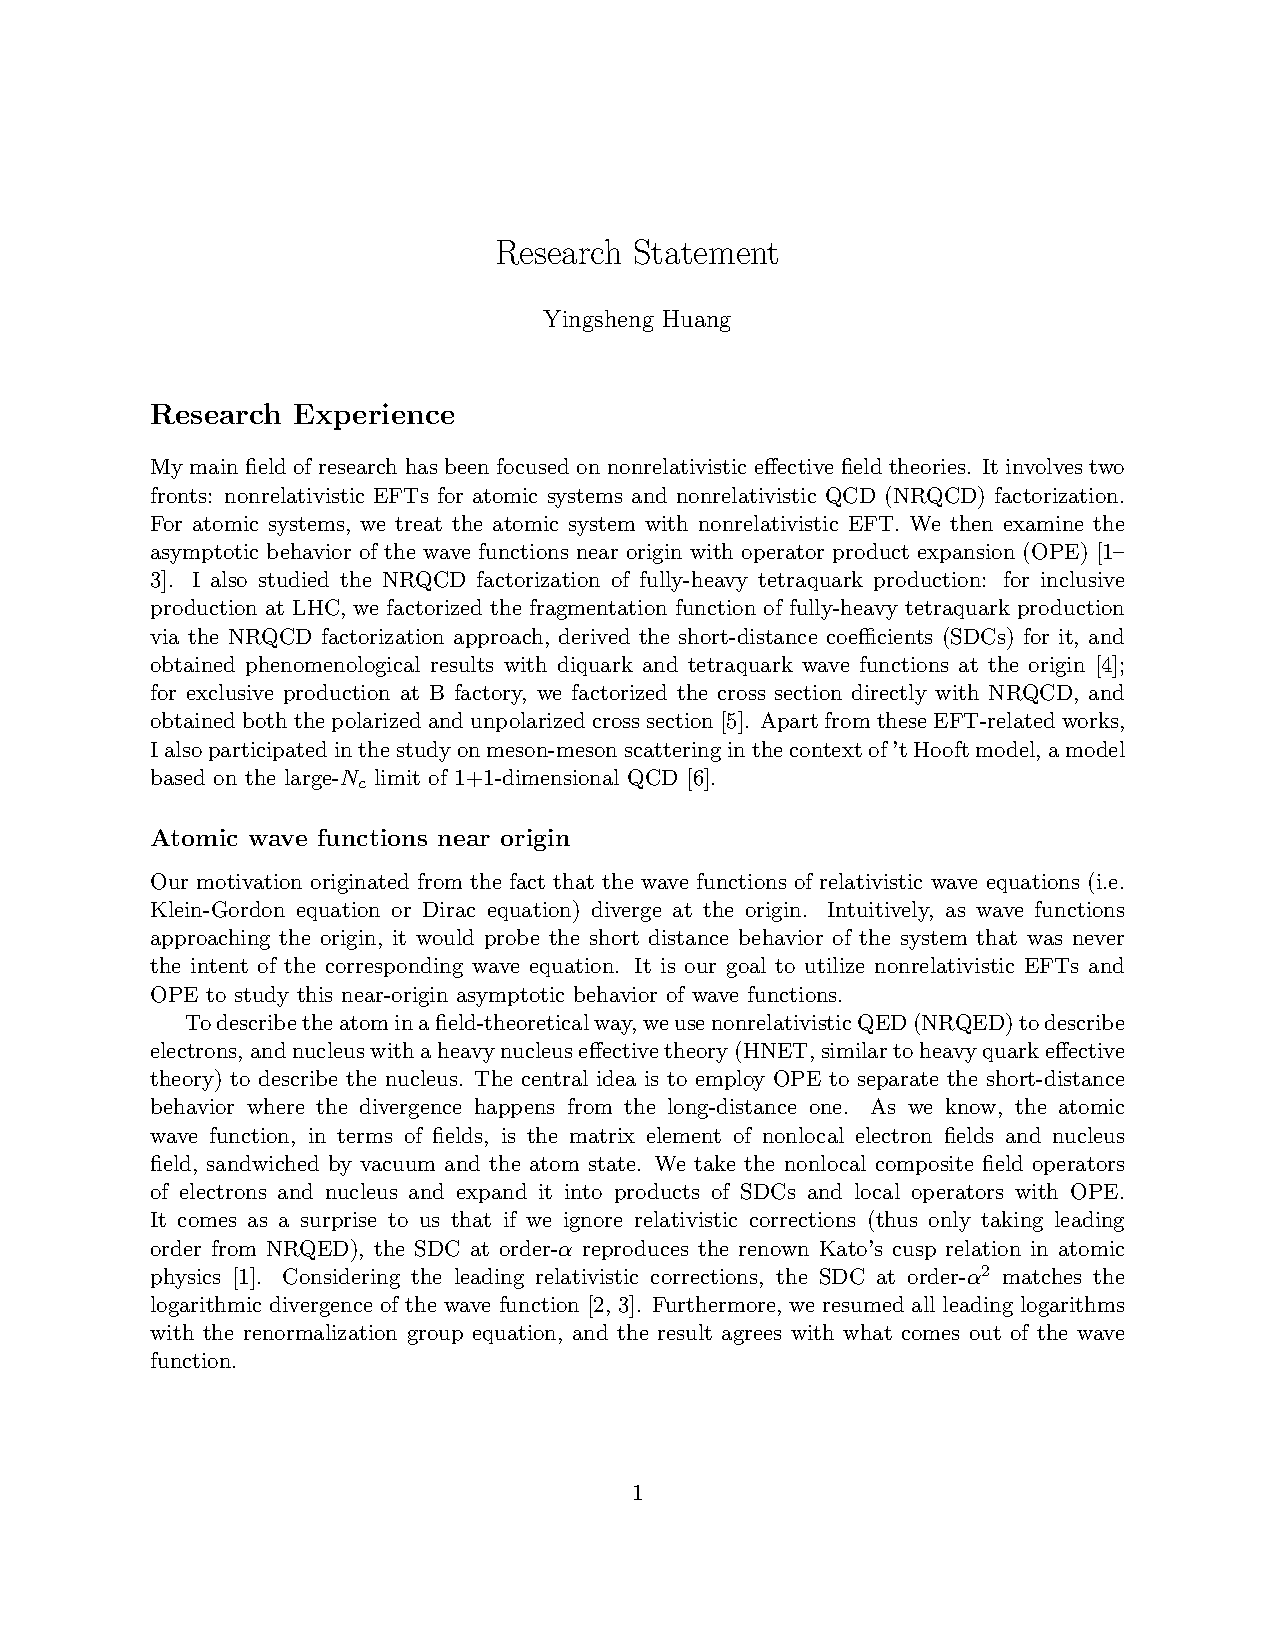
\includepdf[pages=-]{ResearchStatement.pdf}

% Page Two
% \import{sections/}{teaching.tex}
% \sidebyside
%     {\import{sections/}{skills.tex}}
%     {\import{sections/}{languages.tex}}
% \import{sections/}{projects.tex}
% \import{sections/}{awards.tex}
% \import{sections/}{extracurricular.tex}

\end{document}
